\section{Project Proposals}

\begin{frame} \frametitle{Project Proposals}
    % \framesubtitle{02 Maybe Subtitle}
    \begin{block}{Proposals}
        \begin{itemize}
        \item Guitar effect (audio in, audio out)
        \item Automatic music transcriber (audio in, sheet music out)
        \item Differential PCM (signal in, compressed signal out)
        \end{itemize}
    \end{block}
\pause
    \begin{block}{Our Semester}
        \begin{itemize}
        \item Noise suppression (noisy speech in, clean speech out)
        \item Frequency analyzer (music/vibrations in, frequency spectrum/messages out)
        \item AAUSAT radio receiver (radio signal in, bits out)
        \end{itemize}
    \end{block}
\end{frame}

\subsection{Project: Noise Suppression}
\begin{frame}
    \frametitle{Project: Noise Suppression}
    Remove noise from speech in real time.
    \begin{center}
        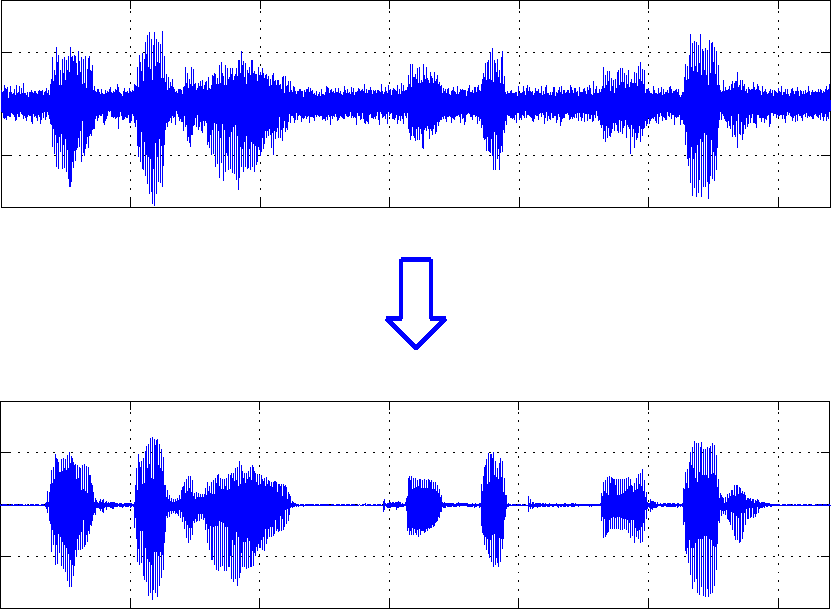
\includegraphics[scale=0.5]{img/noise_1}
    \end{center}
    Speech: \SI{300}{Hz}--\SI{3}{kHz}.
\end{frame}

\subsection{Project: Wind Turbine Analysis}
\begin{frame}
    \frametitle{Project: Wind Turbine Analysis}
    Siemens wind turbine
    \begin{itemize}
    \item Is something broken in the turbine?
    \end{itemize}
    \begin{center}
        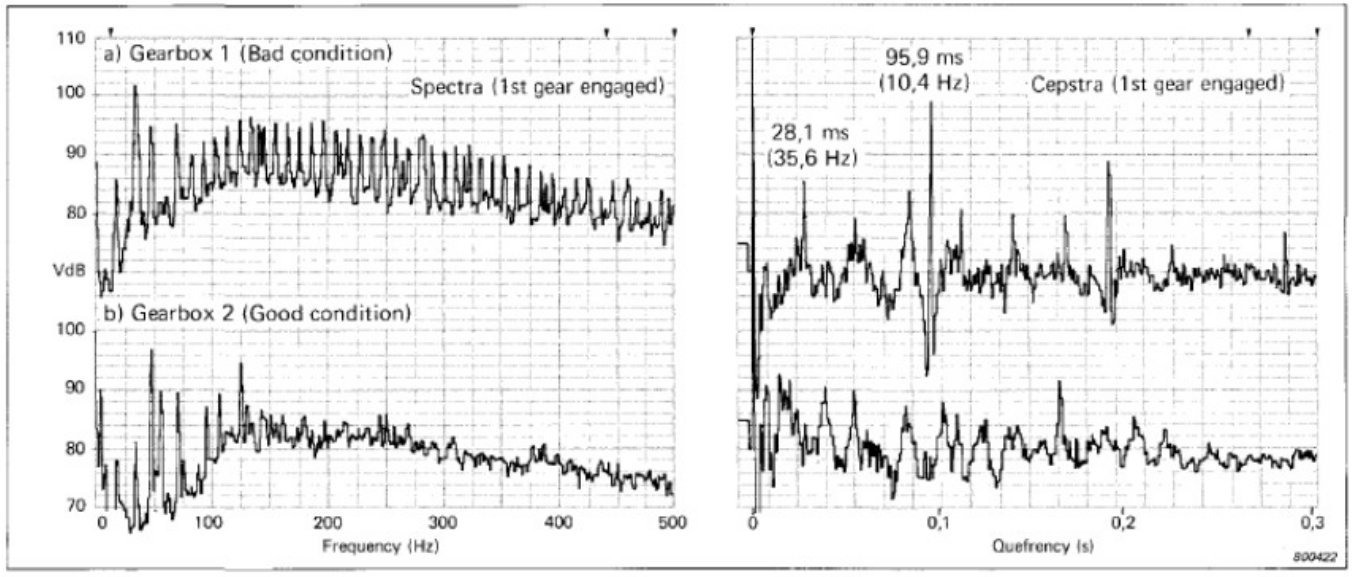
\includegraphics[width=\linewidth]{img/wind_1}
    \end{center}
    Accelerometer input, vibrations analysis.
\end{frame}

\section{Project: AAUSAT Radio Receiver}
\begin{frame}
    \frametitle{Project: AAUSAT Radio Receiver}
    Receive databits from AAUSAT3/4.    
    \begin{center}
        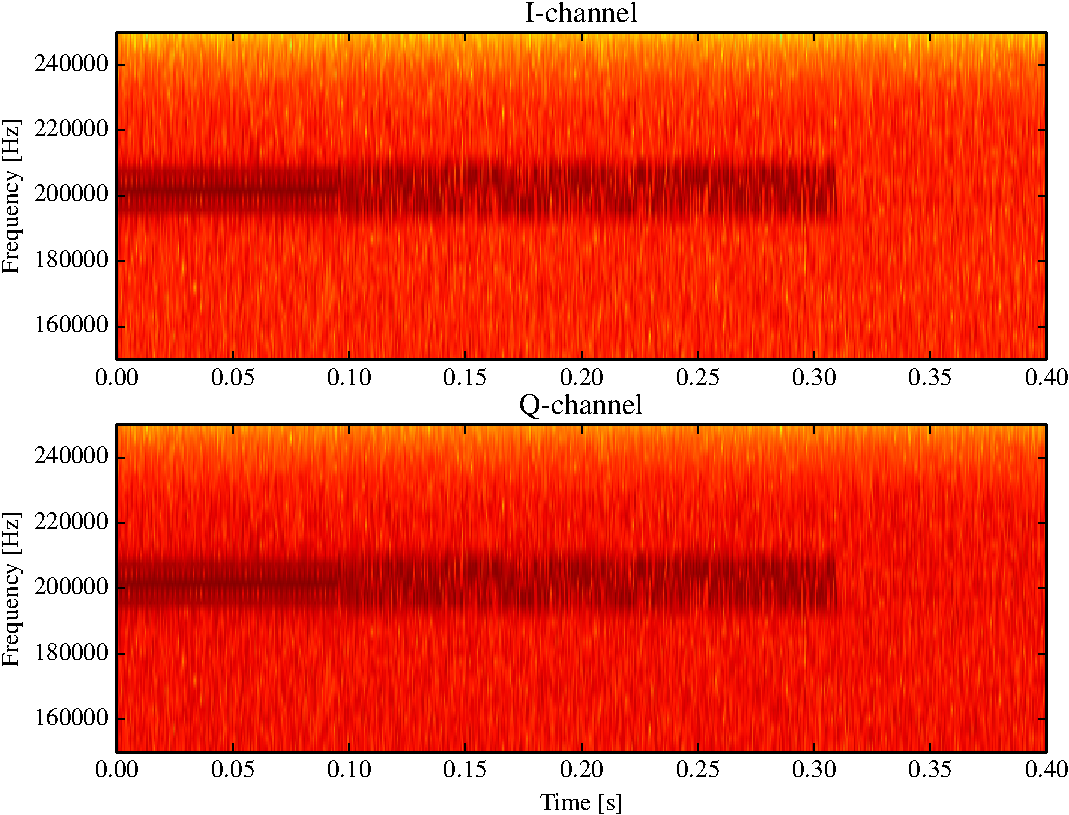
\includegraphics[scale=0.5]{img/specgram_nofilter_zoom_medium}
    \end{center}
\end{frame}

\subsection{Hardware}
\begin{frame}
    \frametitle{Hardware and Software}
    \begin{block}{Hardware}
        \begin{itemize}
        \item Analog Devices Blackfin DSP
        \item (Texas Instruments DSP)
        \item \SI{16}{bit} -- only integers!
        \end{itemize}
    \end{block}

    \pause
    \begin{block}{Software}
        \begin{itemize}
        \item Software for hardware people!
        \item MATLAB for simulation
        \item C + Assembly for implementation
        \item \texttt{float} $\rightarrow$ \texttt{int}
        \end{itemize}
    \end{block}
\end{frame}

\begin{frame}[plain]
    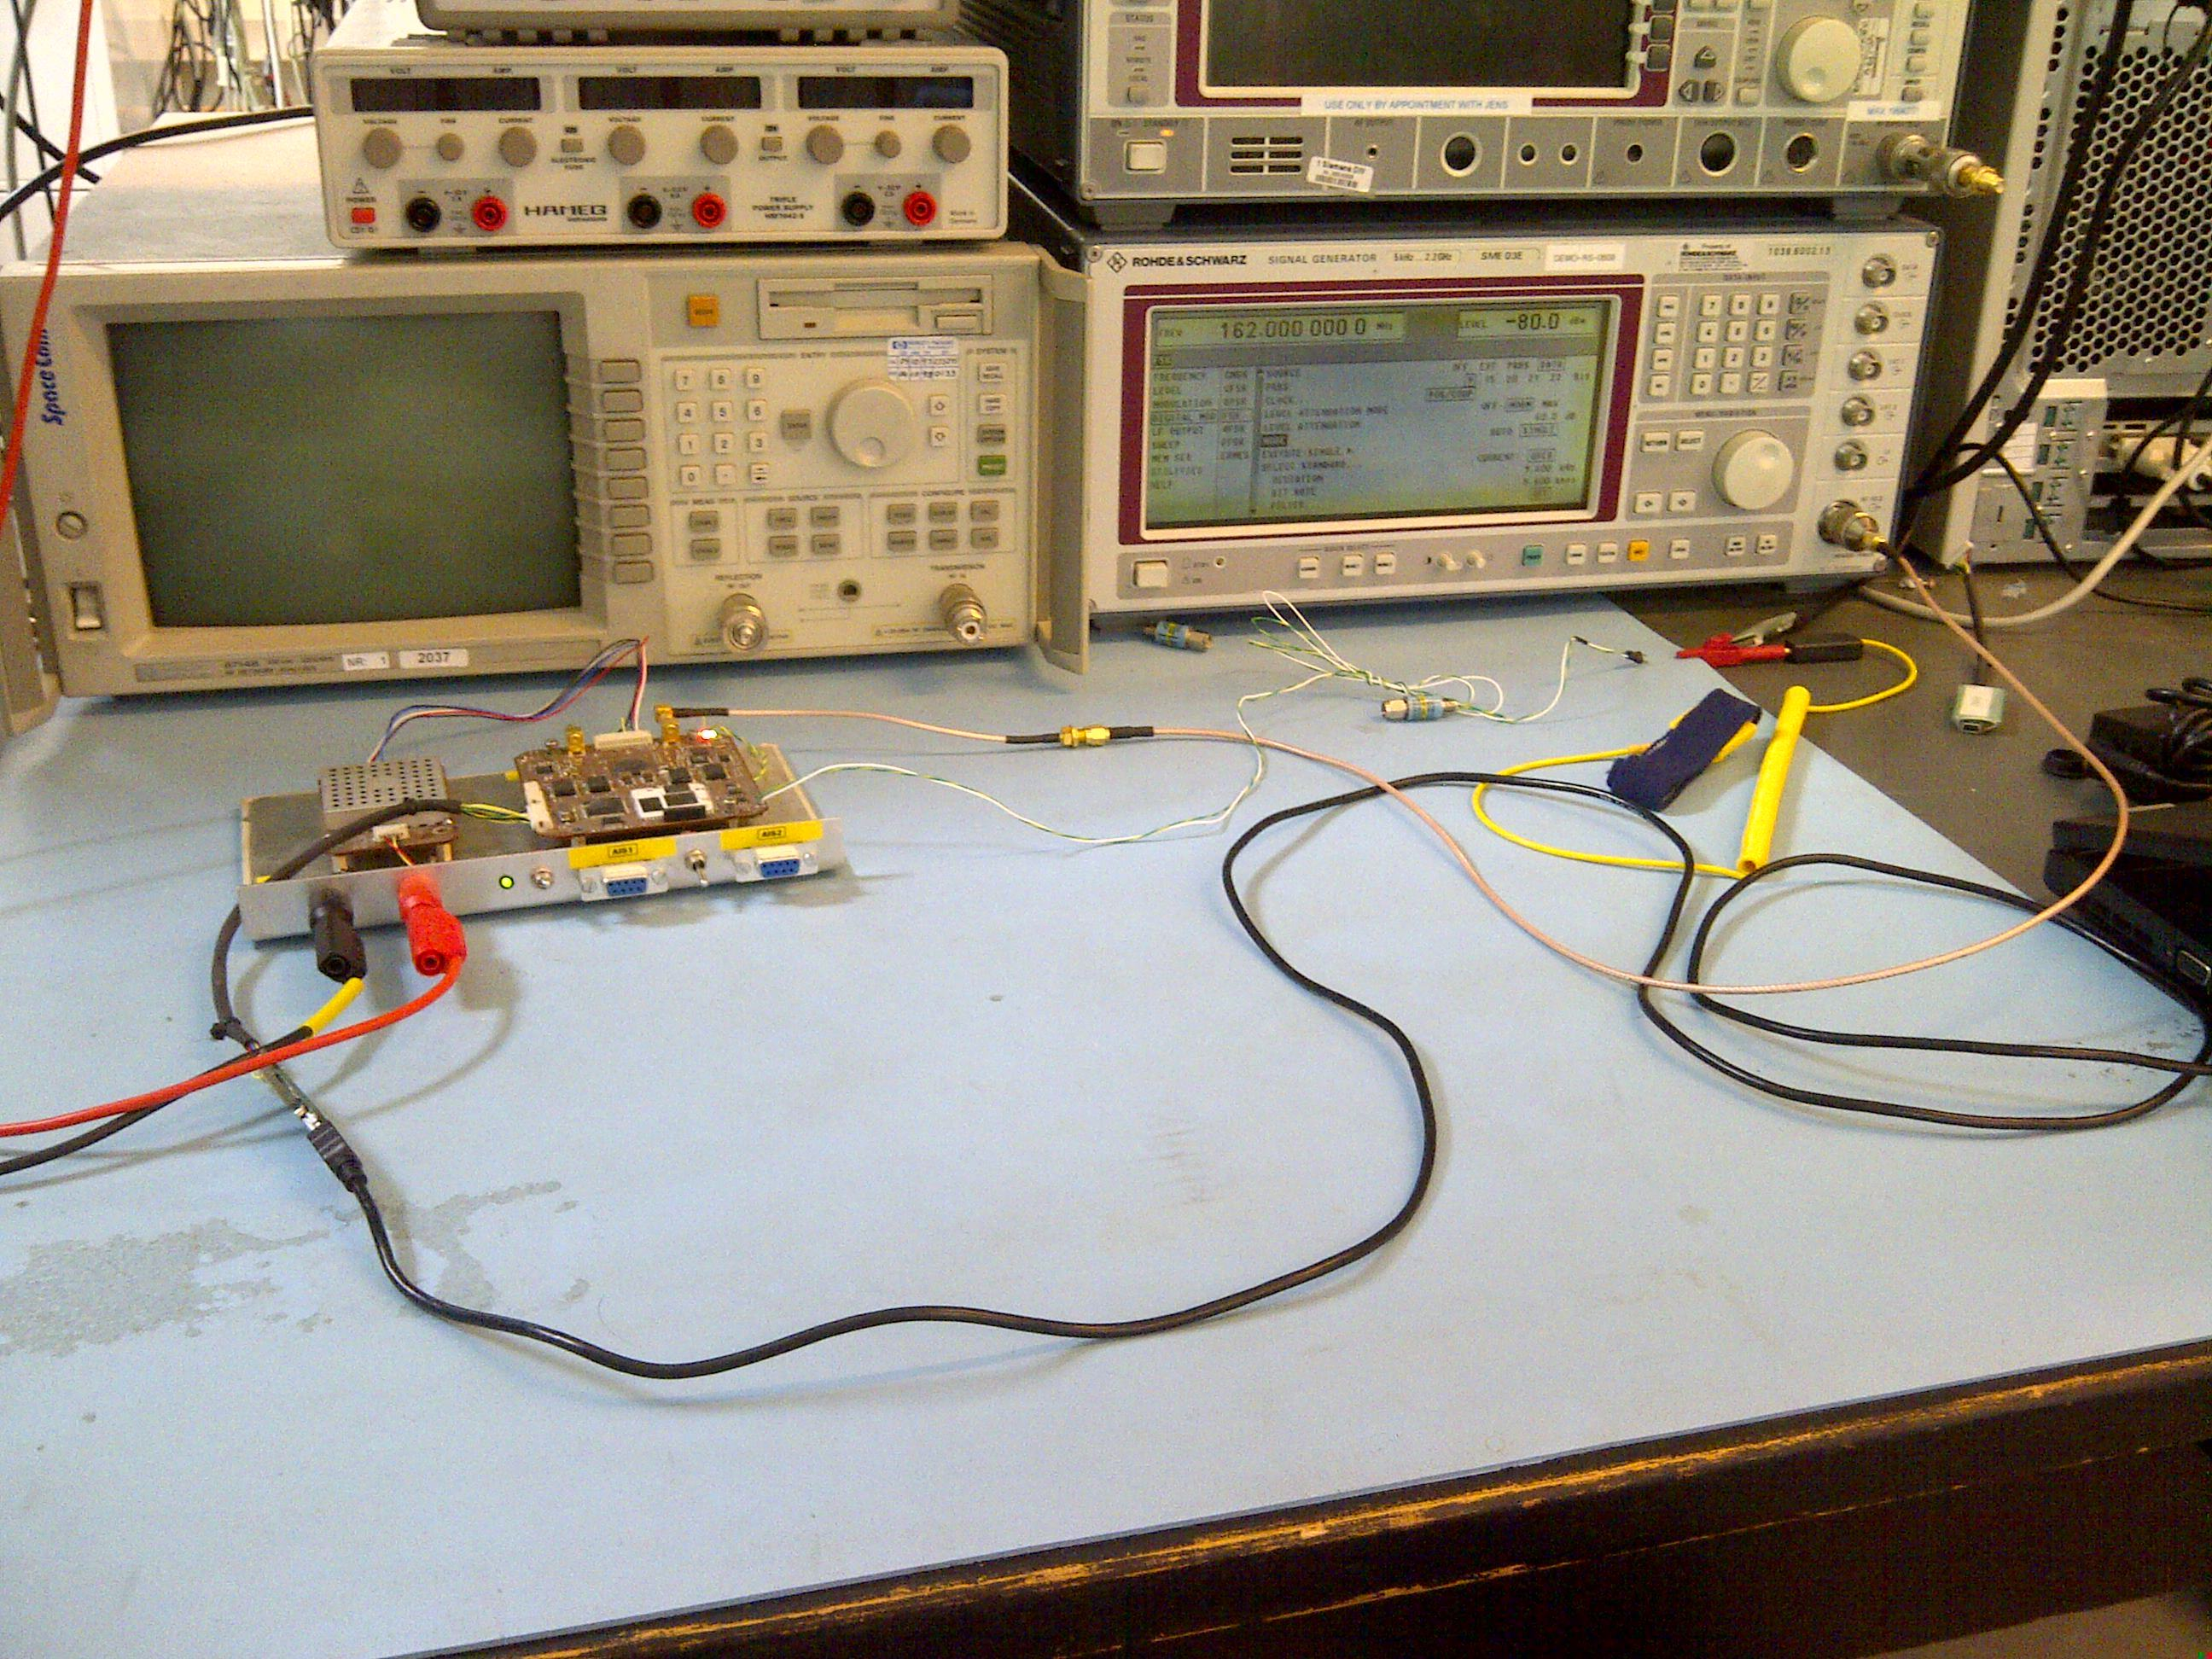
\includegraphics[width=0.92\paperwidth]{img/sdr_3}
\end{frame}
\begin{frame}[plain]
    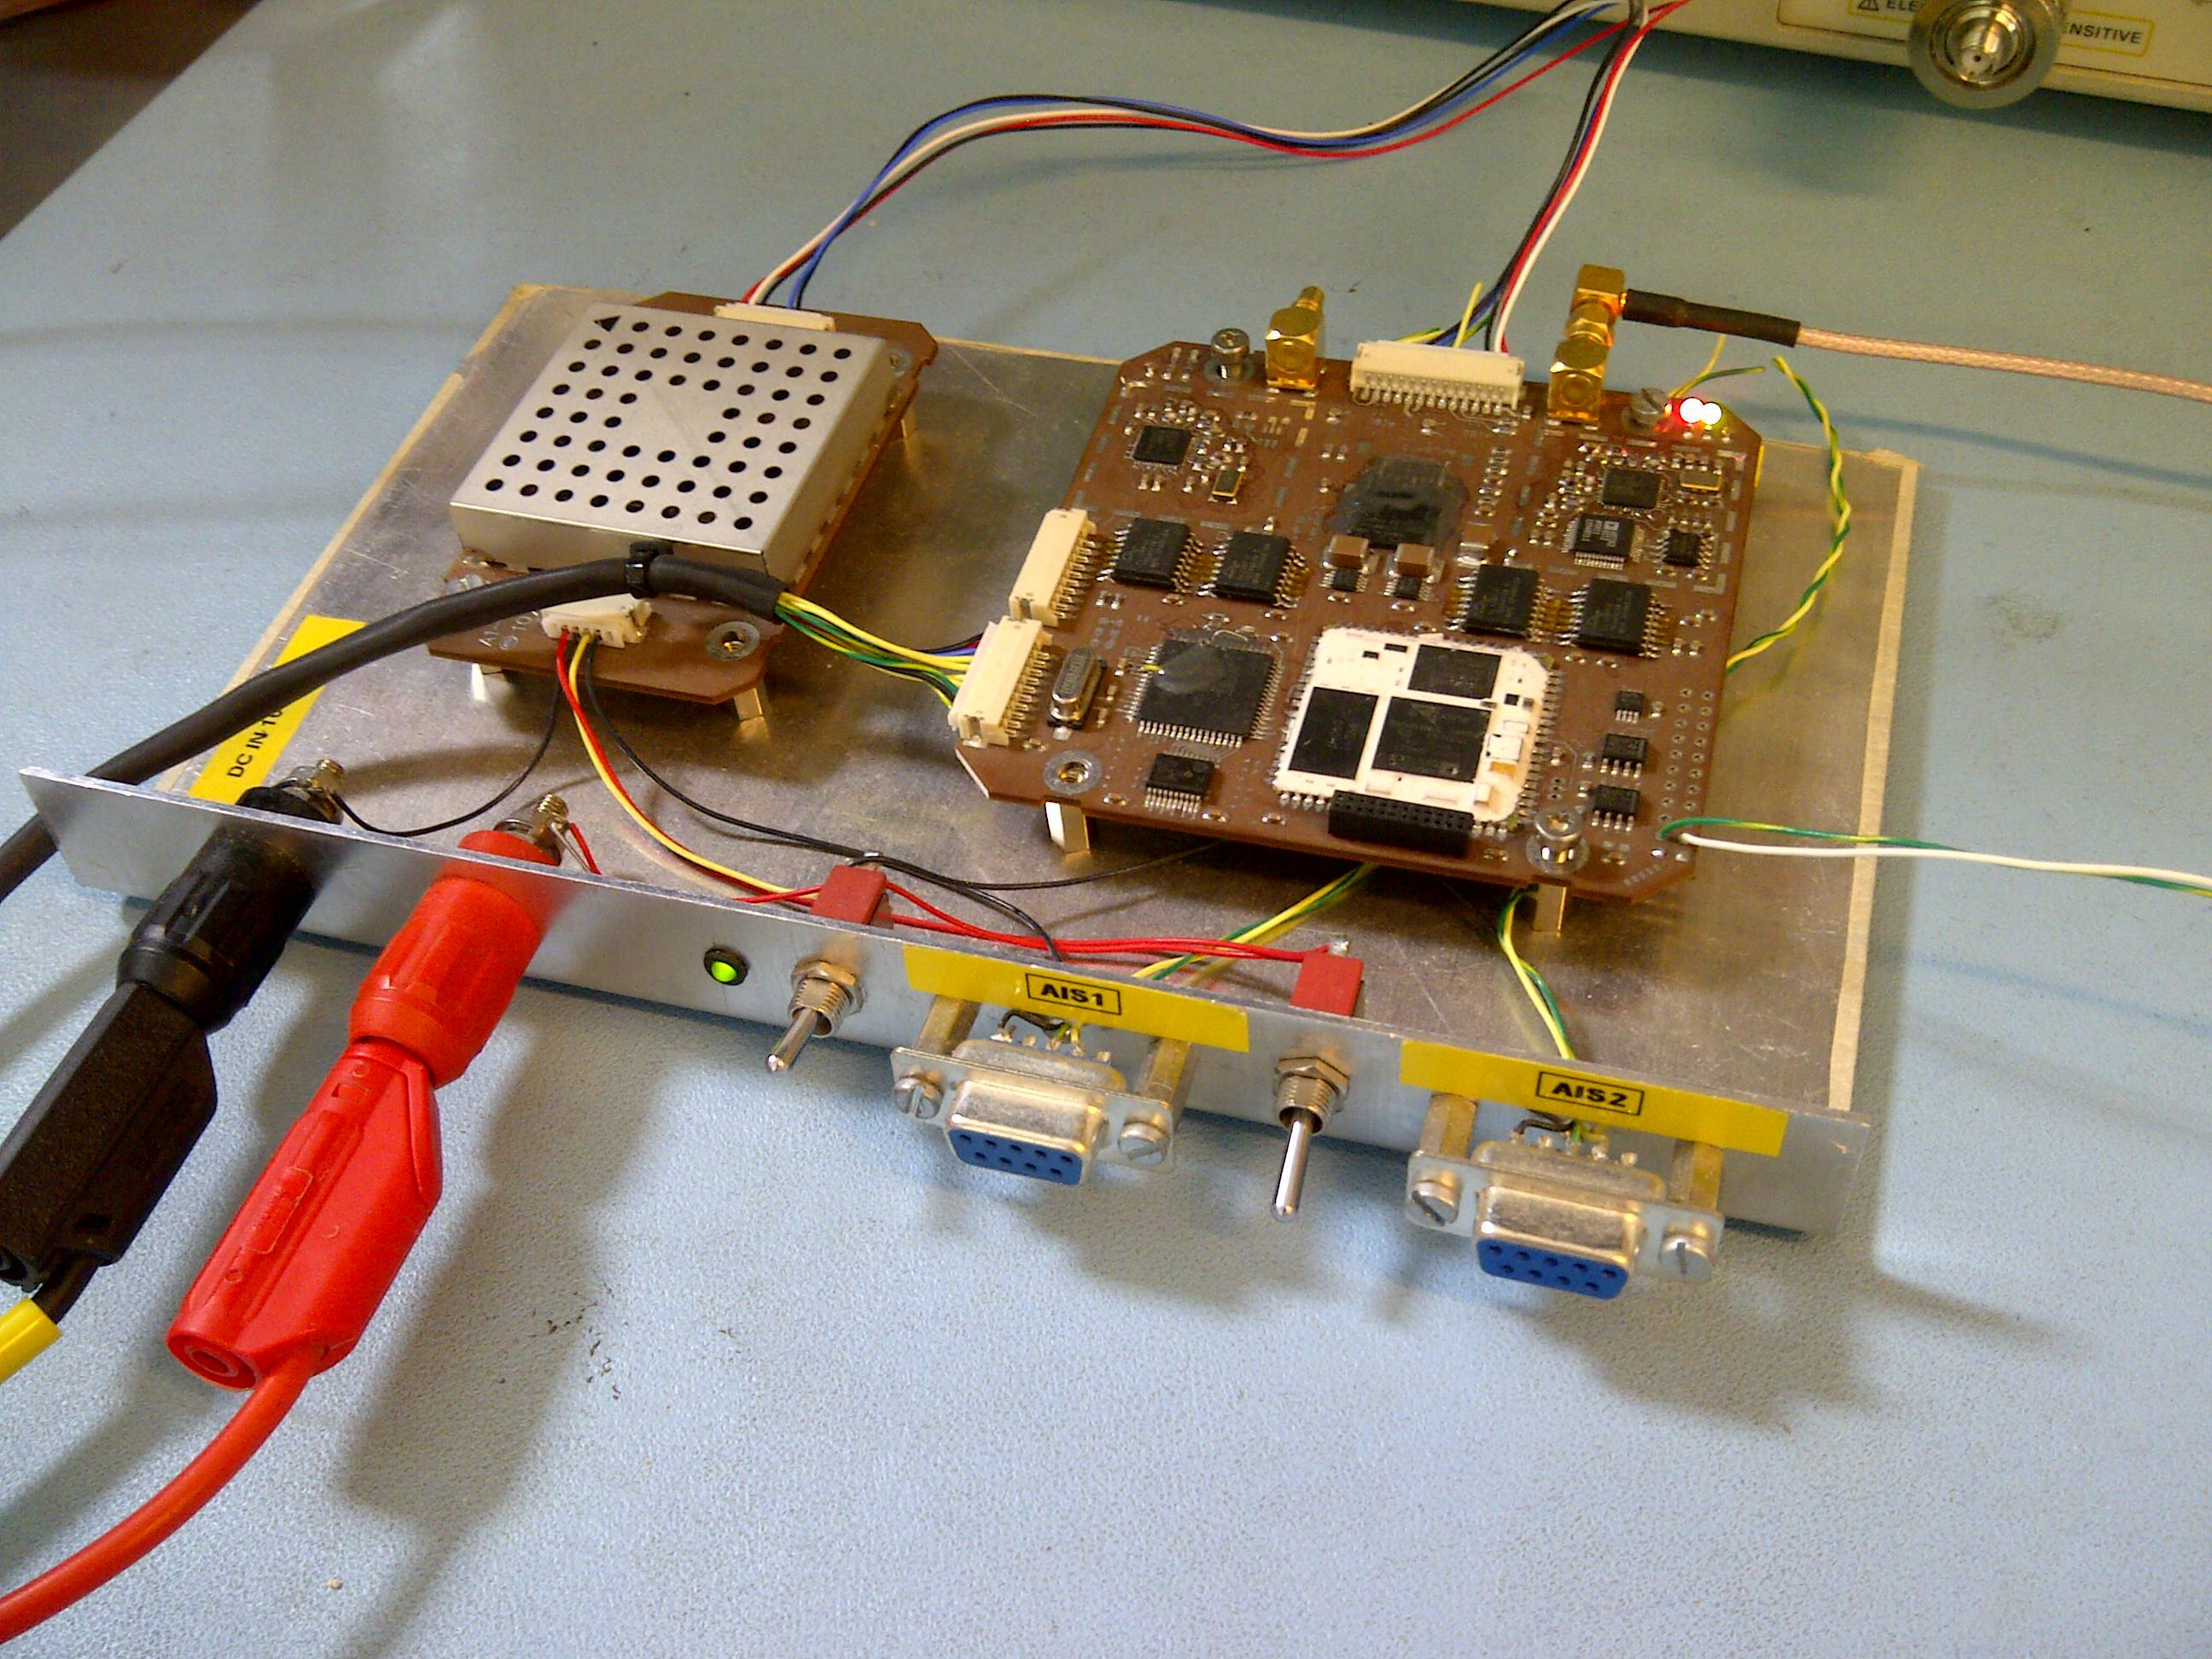
\includegraphics[width=0.92\paperwidth]{img/sdr_2}
\end{frame}


\subsection{Sampling}
\begin{frame}
    \frametitle{Sampling}
    \begin{center}
        \includegraphics{img/sdr_1}
    \end{center}
\end{frame}
